% !TEX root = ../Coherence.tex

\section{Perspectives}

%%%%%%%%%%%%%%%%%%%%%%%%%%%%%%%%%%%%%

\subsection{Further applications} 
\label{sec:further}
One can also use the same strategy to prove coherence for \emph{unital} non-symmetric monoidal categories, using the unital associahedra of F. Muro and A. Tonks \cite{muroUnitalAssociahedra2014}.

It is natural to ask if the construction of unital associahedra could be extended to the permutoassociahedra, in such a way as to provide a topological proof of coherence for unital symmetric monoidal categories. 
The question of the existence of these constructions at the operadic level (i.e. does there exist unital operahedra, symmetric operahedra, and unital symmetric operahedra?) is, to our knowledge, still open as well. 

Another immediate application of \cref{thm:top-coherence} is the coherence of strong non-symmetric monoidal functors between non-symmetric monoidal categories \cite{epsteinFunctorsTensoredCategories1966}. 
The corresponding topological objects are in this case the family of multiplihedra \cite{Stasheff70,Forcey08}.
The generalization to strong morphisms between non-symmetric categorified operads also goes through, involving this time the family of multiploperahedra described at the end of the introduction in \cite{MazuirLA22}.

In the same spirit as in \cref{thm:coherence-operahedra}, one could obtain coherence results for categorifications of many operad-like structures, for instance the ones described in \cite{BMO20}: categorified modular operads, wheeled properads, and permutads (shuffle algebras), among others.
In order to treat cyclic and symmetric structures, one could take inspiration from the reduction process followed in \cite{curienCategorifiedCyclicOperads2020} for the case of cyclic symmetric categorified operads.

\subsection{Higher categories} 
\label{sec:higher}
\cref{thm:top-coherence} demonstrates that, in the case of monoidal categories, coherence is equivalent to the vanishing of the first homotopy groups of the associahedra. 
Since the associahedra are contractible, and therefore all their homotopy groups vanish, one could hope for a topological proof of higher dimensional coherence theorems.
Seeing a monoidal category as a bicategory with one object, one can ask about a coherence theorem for tricategories with one object. 
A first look at the diagrams in the beginning of \cite[Section 2]{gordonCoherenceTricategories1995} suggests that such a theorem should be at least related to the vanishing of the second homotopy groups of the associahedra.  
To formulate higher dimensional statements, one needs a good structure of pasting scheme on each associahedron, which is the subject of ongoing work \cite{AMMLA}. 

Recent results of S. Barkan provide evidence for these higher dimensional statements, in the context of $\infty$-operads \cite{barkanArityApproximationInfty2022}.
In this vein, it seems likely that the present results could be interpreted as a strict version and a special case of \cite[Theorem B]{barkanArityApproximationInfty2022}. 
It would be interesting to see how the permutoassociahedra arise in the strictification process, and how they are related to operadic partition complexes.  

\correction{Add Kapranov--Voevodsky one dimension higher; autre reference ou la correspondance semble etre faite}


\newpage 

\begin{figure}[h!]
\begin{center}
\resizebox{0.8\linewidth}{!}{
 \begin{tikzpicture}[scale=6.5]
    \node (P1) at (0,1) {$(A \otimes B) \otimes C$};
    \node (P2) at (-0.5,0.866) {$A \otimes (B \otimes C)$};
    \node (P3) at (-0.866,0.5) {$A \otimes (C \otimes B)$};
    \node (P4) at (-1,0) {$(A \otimes C) \otimes B$};
    \node (P5) at (-0.866,-0.5) {$(C \otimes A) \otimes B$} ;
    \node (P6) at (-0.5,-0.866) {$C \otimes (A \otimes B)$};
    \node (P7) at (0,-1) {$C \otimes (B \otimes A)$};
    \node (P8) at (0.5,-0.866) {$(C \otimes B) \otimes A$};
    \node (P9) at (0.866,-0.5) {$(B \otimes C) \otimes A$};
    \node (P10) at (1,0) {$B \otimes (C \otimes A)$};
    \node (P11) at (0.866,0.5) {$B \otimes (A \otimes C)$} ;
    \node (P12) at (0.5,0.866) {$(B \otimes A) \otimes C$};
    \draw[->] (P1)--(P2) node[midway,above left] {$\alpha$};
    \draw[->] (P2)--(P3) node[midway,above left] {$\beta$};
    \draw[->] (P3)--(P4) node[midway,above left] {$\kappa$};
    \draw[->] (P4)--(P5) node[midway,below left] {$\theta$};
    \draw[->] (P5)--(P6) node[midway,below left] {$\mu$};
    \draw[->] (P6)--(P7) node[midway,below left] {$\beta$};
    \draw[->] (P1)--(P12) node[midway,above right] {$\alpha$};
    \draw[->] (P12)--(P11) node[midway,above right] {$\beta$};
    \draw[->] (P11)--(P10) node[midway,above right] {$\kappa$};
    \draw[->] (P10)--(P9) node[midway,below right] {$\theta$};
    \draw[->] (P9)--(P8) node[midway,below right] {$\mu$};
    \draw[->] (P8)--(P7) node[midway,below right] {$\beta$};
    \draw[->,dashed] (P2)--(P9) node[midway,above right] {$\alpha$};
    \draw[->,dashed] (P3)--(P8) node[midway,below left] {$\beta$};
\end{tikzpicture}} 
\end{center}
\caption{FIgure}
\label{fig:dodecagon}
\end{figure}


\begin{center}
\resizebox{0.5\linewidth}{!}{
    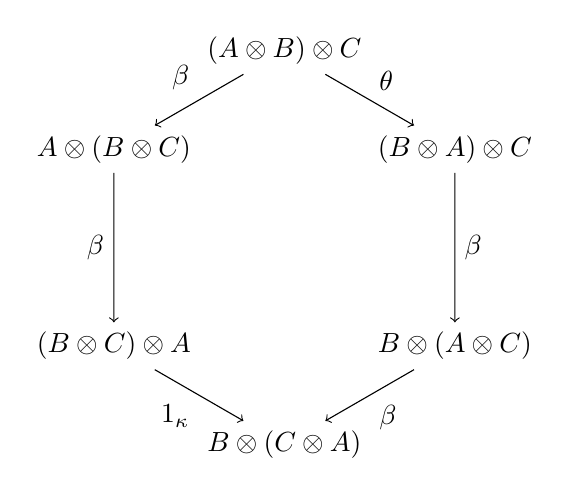
\begin{tikzpicture}[scale=2.5]
    \node (P1) at (0,1) {$(A\otimes B) \otimes C$};
    \node (P2) at (-0.866,0.5) {$A\otimes (B \otimes C)$};
    \node (P3) at (-0.866,-0.5) {$(B \otimes C) \otimes A$};
    \node (P4) at (0,-1) {$B \otimes (C \otimes A)$};
    \node (P5) at (0.866,0.5) {$(B \otimes A) \otimes C$} ;
    \node (P6) at (0.866,-0.5) {$B \otimes (A \otimes C)$};
    \draw[->] (P1)--(P2) node[midway,above left] {$\beta$};
    \draw[->] (P2)--(P3) node[midway,left] {$\beta$};
    \draw[->] (P3)--(P4) node[midway,below left] {$1_\kappa$};
    \draw[->] (P1)--(P5) node[midway,above right] {$\theta$};
    \draw[->] (P5)--(P6) node[midway,right] {$\beta$};
    \draw[->] (P6)--(P4) node[midway,below right] {$\beta$};
\end{tikzpicture}}
\end{center}


